\documentclass{article}
\usepackage{graphicx} % Required for inserting images
\usepackage{geometry}
\usepackage{amsmath}
\usepackage{amsfonts}
\usepackage{graphicx}
\usepackage{caption}
\usepackage{subcaption}

\geometry{a4paper, margin=1in}
\title{\textbf{LINMA2171} \\ Homework I}
\author{Damien Doat \& Théo André }
\date{\today}

\begin{document}

\maketitle

\hrulefill
\vspace{1cm}

\section*{Projected Gradient Method}
\subsection*{(a) Computation of $\nabla f_{l}(.)$}
\begin{equation*}
\begin{split} 
\nabla f_l(X)_{k,l} & = \frac{\partial}{\partial_{k,l}}\frac{1}{2}\sum_{i=1}^{m}
\sum_{j=1}^{n}(X_{i,j} - Y_{i,j})^2 + \frac{\partial}{\partial_{k,l}}\lambda\sum_{i=2}^{m-1}\sum_{j=2}^{n-1}
(X_{i+1,j} - X_{i,j})^2 + (X_{i,j+1} - X_{i,j})^2 \\
                   & = \frac{1}{2}\sum_{i=1}^{m}\sum_{j=1}^{n}\frac{\partial}{\partial_{k,l}}
(X_{i,j} - Y_{i,j})^2 + \lambda\sum_{i=2}^{m-1}\sum_{j=2}^{n-1}\frac{\partial}{\partial_{k,l}}
(X_{i+1,j} - X_{i,j})^2 + \frac{\partial}{\partial_{k,l}}(X_{i,j+1} - X_{i,j})^2 \\
                   & = (X_{k,l} - Y_{k,l}) + \lambda\Big[2(X_{k,l} - X_{k-1,l}) - 2(X_{k+1,l} - X_{k,l}) 
                   + 2(X_{k,l} - X_{k,l-1}) - 2(X_{k,l+1} - X_{k,l})\Big] \\
                   & = (X_{k,l} - Y_{k,l}) + \lambda\Big[8X_{k,l} - 2X_{k-1,l} - 2X_{k+1,l} 
                   - 2X_{k,l-1} - 2X_{k,l+1}\Big]
\end{split}
\end{equation*}
\\
This is a general expression for the $kl$ component of the gradient, but we give a more precise 
expression hereafter to consider the "corner cases"

$$
\nabla f_l(X)_{k,l} =  
                \begin{cases}
                (X_{k,l} - Y_{k,l})  & \text{if $k=1$ and/or $l=1$} \\
                                   & \text{or if $k=m$ and $l=n$}  \\
                (X_{k,l} - Y_{k,l}) + \lambda [4X_{k,l} - 2X_{k+1,l} - 2X_{k,l+1}]
                & \text{if i=2 and j=2} \\
                (X_{k,l} - Y_{k,l}) + \lambda[6X_{k,l} - 2X_{k+1,l} - 2X_{k,l-1}
                -2X_{k,l+1}]  
                & \text{k=2 and $3\leq l\leq n-1$} \\
                (X_{k,l} - Y_{k,l}) + \lambda[6X_{k,l} - 2X_{k,l+1} - 2X_{k-1,l}
                -2X_{k+1,l}]  
                & \text{l=2 and $3\leq k\leq m-1$} \\
                (X_{k,l} - Y_{k,l}) + \lambda[2X_{k,l} - 2X_{k-1,l}] 
                & \text{k=m and $2\leq l\leq n-1$} \\
                (X_{k,l} - Y_{k,l}) + \lambda[2X_{k,l} - 2X_{k,l-1}] 
                & \text{$l=n$ and $2\leq k\leq m-1$} \\
                (X_{k,l} - Y_{k,l}) + \lambda[8X_{k,l} - 2X_{k-1,l} - 2X_{k+1,l} 
                -2X_{k,l-1} - 2X_{k,l+1}] 
                & \text{else} 
                \end{cases}
$$


\subsection*{(b) $\nabla f_{l}(.)$ $L$-Lipschitz derivation}
We recall that a function $F : \mathbb{R}^n \to \mathbb{R}^n$ is $L$-Lipschitz if there exists 
a constant $L$ such that \\$ ||F(x) - F(y)|| \leq L||x-y|| \quad \forall x,y \in \mathbb{R}^n$. \\
To find L for $\nabla f_l(.)$, we will consider the general case of the derivation above, 
since it will lead to upper bound for the corner cases and we will assume a 0 value for
the terms with out of bounds index. We will also work on the following form to avoid square
roots: $||F(x) - F(y)||^2 \leq L^2||x-y||^2$. \\This leads to:

\begin{align}
||\nabla f_l(X) - \nabla f_l(Y)||^2  & \leq \sum_{i=1}^{m}\sum_{j=1}^{n}\Big(|X_{i,j} - Y_{i,j}| + \lambda\Big[8|X_{i,j}
                      -Y_{i,j}| + 2|X_{i,j+1} - Y_{i,j+1}| \\
                   & \quad \quad + 2|X_{i,j-1} - Y_{i,j-1}| + 
                     2|X_{i+1,j} - Y_{i+1,j}| + 2|X_{i-1,j} - Y_{i-1,j}|\Big]\Big)^2 \\
                   & = \sum_{i=1}^{m}\sum_{j=1}^{n}\Big(|\Delta_{ij}| + \lambda\Big[8|\Delta_{ij}|
                       + 2|\Delta_{i-1,j}| + 2|\Delta_{i+1,j}|
                       + 2|\Delta_{i,j-1}| + 2|\Delta_{i,j+1}|\Big]\Big)^2 \\
                   & \leq 5\sum_{i=1}^{m}\sum_{j=1}^{n}(|\Delta_{i,j}| + 16\lambda|\Delta_{i,j}|)
                       ^2 \\
                   & = \sum_{i=1}^{m}\sum_{j=1}^{n}(\sqrt{5}(1+16\lambda))^2(\Delta_{i,j})^2
\end{align}

\noindent Where we use the fact that $(\alpha_1x_1 + \alpha_2x_2 + \alpha_3x_3)^2 \leq (\alpha_1
+ \alpha_2 + \alpha_3)^2(x_1^2+x_2^2+x_3^3)$ as all alphas are $\geq 0$ to go from
(3) to (4). Then we can identify the Lipschitz constant, $L = \sqrt{5}(1+16\lambda)$. 

\subsection*{(c) $f_{l}(.)$ convexity derivation}
$f_l(.)$ is convex. To show this, we use some basic properties already known:
\begin{enumerate}
\item The norm functions are convex
\item The composed of a convex function with a nondecreasing convex function is
convex
\item The sum of convex functions is convex
\item $g : \mathbb{R} \to \mathbb{R} : t \to t^2$ is convex
\item if $f(x)$ is convex, then $c.f(x)$ is assuming c positive
\end{enumerate}
Then it follows that from 1. and 2. $||X-Y^{(l)}||_{F}^2$ is convex.
Now we show that every term of the regularizer, noted $h$, is convex using the 
definition of convexity: \\
Consider any $X$ and $Y \in [0,255]^{m\times n}$ and $h(Z) = (Z_{i+1,j}-Z_{i,j})^2.
$Then we want to show that
\begin{align*}
h(\alpha X + (1-\alpha)Y) &\leq \alpha h(X) + (1-\alpha)h(Y) \\
(\alpha X_{i+1,j} + (1-\alpha) Y_{i+1,j} - (\alpha X_{i,j} + (1-\alpha)Y_{i,j}))^2
&\leq \alpha (X_{i+1,j}-X_{i,j})^2 + (1-\alpha)(Y_{i+1,j} - Y_{i,j})^2 \\
(\alpha t_1 + (1-\alpha)t_2)^2 &\leq \alpha t_1^2 + (1-\alpha) t_2^2 
\end{align*}
Where we posed $t_1 = (X_{i+1,j} - X_{i,j})$ and $t_2 = (Y_{i+1,j} - Y_{i,j})$. And
since we find the classic definition of the convexity of $t^2$, we have 
that $h(Z)$ is convex. So now we can observe that $f_l(.)$ is the sum of 
weighted convex functions and by 3. and 5., It is also convex.







\subsection*{(d) Implementation of ProjGM}
See file \texttt{code devoir 1.py}. We used numba to accelerate the execution of the code, so 
if you run the program it will take more time at the beginning but then it will be much faster.
\subsection*{(e) Result of PGM}
We applied our code with $\lambda \in \{0.1, 1, 5, 10\}$ and we got the following
images (see next page).
\begin{figure}[h]
  \centering
  \begin{subfigure}[b]{0.48\textwidth}
  \centering
  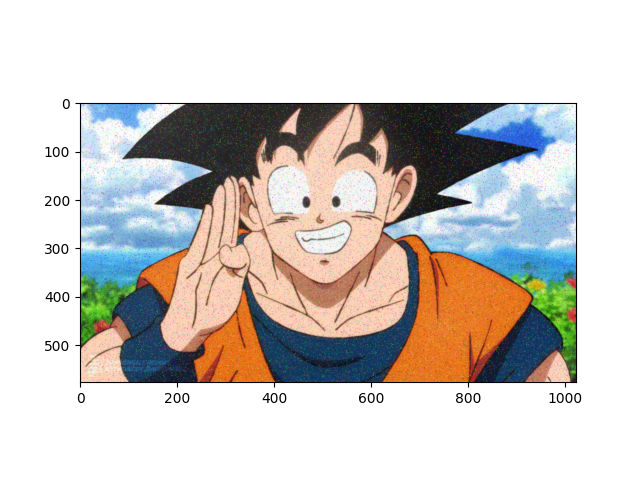
\includegraphics[width=\textwidth]{images/Goku_lambda_0_1.png}
  \caption{$\lambda = 0.1$}
  \label{fig:0.1}
  \end{subfigure}
  \hspace{0.02\textwidth}
  \begin{subfigure}[b]{0.48\textwidth}
  \centering
  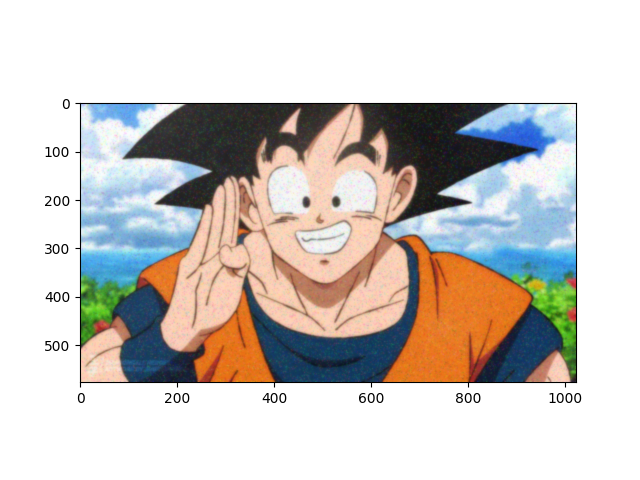
\includegraphics[width=\textwidth]{images/Goku_lambda_1.png}
  \caption{$\lambda = 1$}
  \label{fig:1}
  \end{subfigure}
  \vskip \baselineskip
  \begin{subfigure}[b]{0.48\textwidth}
  \centering
  \includegraphics[width=\textwidth]{images/Goku_lambda_5.png}
  \caption{$\lambda = 5$}
  \label{fig:5}
  \end{subfigure}
  \hspace{0.02\textwidth}
  \begin{subfigure}{0.48\textwidth}
  \centering
  \includegraphics[width=\textwidth]{images/Goku_lambda_10.png}
  \caption{$\lambda = 10$}
  \label{fig:10}
  \end{subfigure}
\end{figure}

\subsection*{(f) Relation between $\lambda$ and the quality}
Based on these results, we can observe that when $\lambda$ is small, then the
regularizer term will have a small impact on the optimization problem. So the
obtained image after solving the problem will be close to the original one, and
exactly the same with $\lambda = 0$. When increasing $\lambda$, the regularizer term
will take more importance and the solution will reduce the difference between the pixels.
It will result in remooving the noise, but a blurred image. 


\section*{Proximal Gradient Method}
\subsection*{(a) Solving SIR model}
See file \texttt{code devoir 1.py} and data.txt. 

\subsection*{(b) Implementation of ProxGM}
See file \texttt{code devoir 1.py}.
\subsection*{(c) SINDy results}
To apply SINDy, we first computed the gradient of $f(\alpha) = \frac{1}{2}||b^{(l)} -
\Theta\alpha||_2^2$ and then $L$ a Lipschitz constant of the gradient:
$$ \nabla f(\alpha)_k = \sum_{i=1}^{m}\theta_{i,k}(-b_i + \sum_{j=1}^{p}\alpha_j
\theta_{i,j})$$
\begin{align*}
||\nabla f(\alpha) - \nabla f(\beta)||^2 & = \sum_{k=1}^{p}\Big(\sum_{i=1}^{m}
  \theta_{i,k} \sum_{i=1}^{p}(\alpha_j-\beta_j)\theta_{i,j}\Big)^2 \\
                                       & \leq \sum_{k=1}^{p}\Big(\sum_{i=1}^{m}
  |\theta_{i,k}| \sum_{i=1}^{p}|\alpha_j-\beta_j||\theta_{i,j}|\Big)^2 \\
                                       & \leq p\bar{\theta}^2\Big(\sum_{i=1}^{m}\sum
                                       _{j=1}^{p}|\alpha_j - \beta_j|\Big)^2 \\
                                       & \leq p^2\bar{\theta}^2m^2\sum_{j=1}^{p}(\alpha_j -
                                       \beta_j)^2
\end{align*}
Where $\bar{\theta}$ represents the maximum entry of the $\Theta$ matrix we can identify a 
Lipschitz constant, $L = p\bar{\theta}m$
Then we solve (5) from the homework statement with our implementation (b) and we get the 
following coefficients: \\
\[
\alpha^{(1)} = \begin{bmatrix}
-8.54 \times 10^{-4} \\
0.0 \\
1.75 \times 10^{-5} \\
-1.94 \times 10^{-1} \\
0.0
\end{bmatrix}
\quad
\alpha^{(2)} = \begin{bmatrix}
1.05 \times 10^{-3} \\
-4.14 \times 10^{-2} \\
0.0 \\
1.77 \times 10^{-1} \\
-9.87 \times 10^{-3}
\end{bmatrix}
\quad
\alpha^{(3)} = \begin{bmatrix}
2.65 \times 10^{-4} \\
4.96 \times 10^{-2} \\
-2.29 \times 10^{-5} \\
0.0 \\
0.0
\end{bmatrix}
\]
Removing the terms smaller than $10^{-3}$, we get the following system of equations:
\begin{align*}
\dot{x}_1(t) &= -0.194x_1(t)x_2(t) \\
\dot{x}_2(t) &= 0.001x_1(t) -0.041x2(t) + 0.177x_1(t)x_2(t) -0.009x_2(t)x_3(t) \\
\dot{x}_3(t) &= 0.049x_2(t)
\end{align*}
We can see that SINDy is working well and giving good results.
\begin{figure}[h]
\centering 
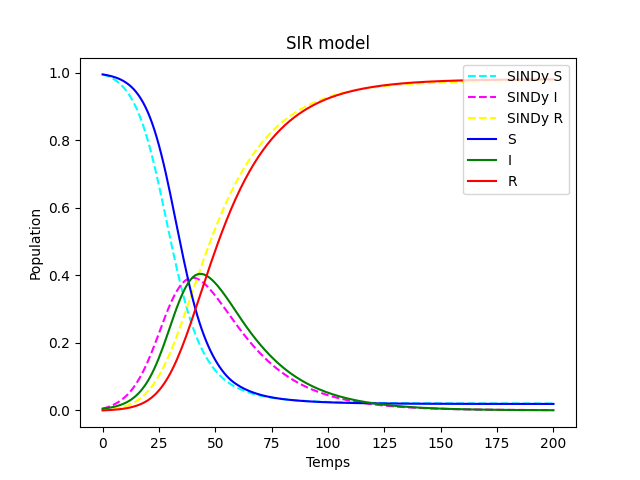
\includegraphics[width=0.8\textwidth]{images/SIR.png}
\caption{SINDy results comparison}
\label{fig:SIR}
\end{figure}
\subsection*{(d) Impact of $\lambda$ on SINDy}
When running SYNDy with $\lambda = 10^{-4}$ we can retireve more
precisely the coefficients of the SIR model:
\[
\alpha^{(1)} = \begin{bmatrix}
-5.11 \times 10^{-4} \\
3.53 \times 10^{-3} \\
0.0  \\
-2.04 \times 10^{-1} \\
-3.53 \times 10^{-3}
\end{bmatrix}
\quad
\alpha^{(2)} = \begin{bmatrix}
4.82 \times 10^{-4} \\
-5.27 \times 10^{-2} \\
-2.77 \times 10^{-6} \\
2.0 \times 10^{-1} \\
4.13 \times 10^{-3}
\end{bmatrix}
\quad
\alpha^{(3)} = \begin{bmatrix}
4.02 \times 10^{-5} \\
4.88 \times 10^{-2} \\
-2.49 \times 10^{-6} \\
4.3 \times 10^{-3} \\
0.0
\end{bmatrix}
\]
However when increasing $\lambda$ to $10^{-2}$ or $10^{-1}$, we get very bad results as shown in the following
figure. This highlights the importance of chossing a nice value for $\lambda$
\begin{figure}[h]
\centering 
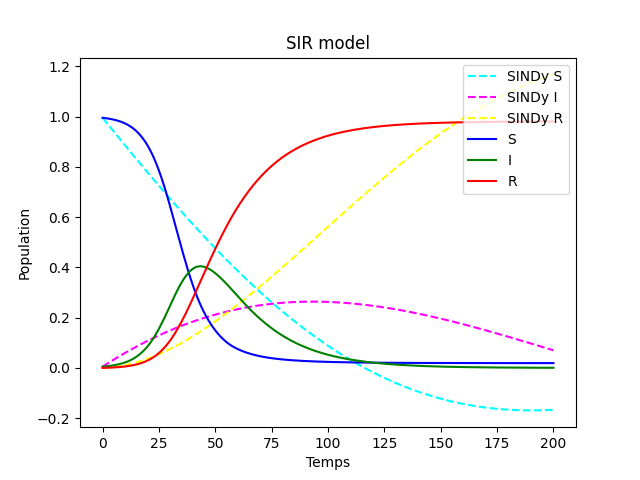
\includegraphics[width=0.8\textwidth]{images/SIR_lambd_1e-1.png}
\caption{SINDy $\lambda=0.1$}
\label{fig:SIR_bad}
\end{figure}
\end{document}
